% % \section{Sensitivity to Parts of the LLM Prompt Being Changed} \textcolor{red}{Move to Appendix?}

% We slightly modified the prompt from the preceding section to check for sensitivity to specific parts of the LLM prompt being removed or modified.
% % For sensitivity analyses with respect to the quality of different prompt strategies for extracting textual time-series (\texttt{DeepSeek R1}) from PMOA case reports, we omitted selected sections of the LLM query prompt
% % (see Appendix \ref{apd:extraction_prompt} for the full prompt).
% This led to the following variants:
% \begin{enumerate}
%     \item \textbf{No changes}: Original LLM query prompt. % for \texttt{DeepSeek-R1}.
    
%     \item \textbf{No role:} Remove the initial sentence \texttt{"You are a physician."}.
    
%     \item \textbf{Zero-shot prompting:} Remove the example case report and textual time-series from the prompt. \\
%     %\item \textbf{No conjunction expansion:} 
%     \textcolor{teal}{\texttt{An 18-year-old male was admitted to ..}}\\
%     "Let's find the locations of event in the case report, it shows that ... then the output should look like:"\\
%     \texttt{18 years old | 0 \\
%     male | 0 \\
%     ..}

%     \item \textbf{No conjunction expansion:} Remove the following sentence from the prompt: \texttt{"Separate conjunctive phrases into its component events and assign them the same timestamp (for example, separation of ‘fever and rash’ into 2 events: ‘fever’ and ‘rash’)"}
    
%     \item \textbf{Interval:} A query was added to the prompt for extracting the time interval (start and end time of clinical events). The original prompt’s instructions and few-shot examples were modified accordingly. 
    
%     \item \textbf{Interval + Type:} A query was added to the prompt for extracting the time interval and i2b2
%     event type (Interval+Type), where event type is one of: Factual, Possible, Hypothetical, Conditional, Negated, Historical, Uncertain. The original prompt’s instructions and few-shot examples were modified accordingly. 
% \end{enumerate}


\begin{figure}[!thbp]
\centering
    \begin{minipage}[t]{0.242\textwidth}
    \centering
    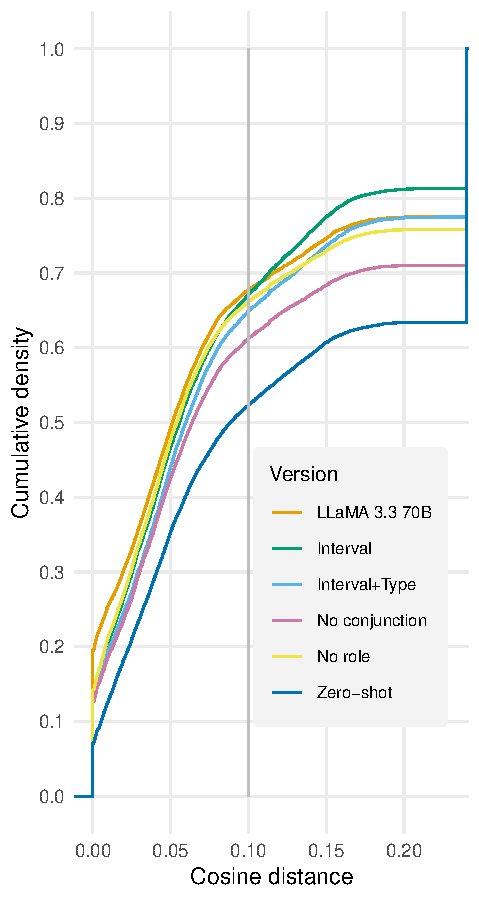
\includegraphics[page=1, width=\linewidth]{Plots_tables/prompt_ablation_updated_figure.pdf}
    \end{minipage}
    \hfill
    \begin{minipage}[t]{0.242\textwidth}
    \centering
    \includegraphics[page=2, width=\linewidth]{Plots_tables/prompt_ablation_updated_figure.pdf}
    \end{minipage}
    \hfill
    \begin{minipage}[t]{0.242\textwidth}
    \centering
    \includegraphics[page=3, width=\linewidth]{Plots_tables/prompt_ablation_updated_figure.pdf}
    \end{minipage}
    \hfill
    \begin{minipage}[t]{0.242\textwidth}
    \centering
    \includegraphics[page=4, width=\linewidth]{Plots_tables/prompt_ablation_updated_figure.pdf}
    \end{minipage}
    \caption{Comparison of \texttt{Llama 3.3 70B} prompt ablation and variant methods for extracting temporal clinical events from case reports. From left to right: (\textbf{A}) event match cumulative distribution function, (\textbf{B}) concordance box plots, (\textbf{C}) time discrepancy from manual annotation timestamps among matched events (overall), and (\textbf{D}) time discrepancy disaggregated by clinician annotator timestamp (time from presentation).}
    \label{fig:prompt_ablation}
    \vspace{-5mm}
\end{figure}
